\documentclass[a4paper]{article}

\usepackage{amsfonts, amsmath, amssymb, amsthm}
\usepackage{graphicx}
\usepackage{fullpage}
\usepackage{float}

\usepackage{tikz}
\usetikzlibrary{calc}

\newtheorem{lemma}{Lemma}
\newtheorem{theorem}{Theorem}
\newtheorem{corollary}{Corollary}
\newtheorem{conjecture}{Conjecture}

\newcommand{\Z}{\mathbb{Z}}
\newcommand{\N}{\mathbb{N}}
\renewcommand{\qedsymbol}{$\blacksquare$}
\newcommand{\abs}[1]{\left| #1 \right|}
\renewcommand{\dim}[1]{\text{dim}\left( #1 \right)}

\setlength{\parindent}{0em}
\setlength{\parskip}{1em}

\begin{document}
	\title{The Graph Diameter of $n \times n$ \textit{Lights Out}}
	\author{William Boyles}
	\date{\today}
	\maketitle
	
	\section{Introduction}
	Consider a simple undirected graph $G=(V,E)$ where each vertex consists of a clickable light.
	Clicking any vertex $v$ toggles the on/off state of $v$ and its neighbors, which Sutner calls a $\sigma$-rule.
	Starting from an initial configuration of the lights, we seek a subset of vertices such that clicking each vertex minimizes the number of on lights.
	We consider an initial configuration solvable if the minimal number of on lights is 0.
	We pose the Min Moves Problem (MMP):
	\begin{quote}
		For $G$, what is the most number of vertices needed to solve any solvable initial configuration?
	\end{quote}
	Eriksson, Eriksson, and Sjöstrand show in \cite{ERIKSSON2001357} that the answer to the MMP is $\abs{V}$ if and only $G$ the number of perfect matchings in $G$ is odd.
	Focusing their attention to when $G$ is an $n \times n$ grid graph, Anderson and Feil show in \cite{anderson_feil} that the function $\Phi: P(V) \to P(V)$ that maps which buttons are pressed to which lights turn on can be described as a $\abs{V} \times \abs{V}$ matrix, and when $\Phi$ is a bijection (i.e. ``nullity'' $\dim{\ker{\Phi}}$ is 0), the answer to the MMP is $\abs{V}$.
	
	Generalizing a technique provided by Scherphuis in \cite{jaap} to solve the MMP for a $5 \times 5$ grid, we provide a solution to the MMP for all grids of size $(6k-1) \times (6k-1)$ with nullity 2.
	We conjecture that this solves the MMP for all nullity 2 grids.
	This solution yields an upper bound to the MMP for all grids of size $(6k-1) \times (6k-1)$, regardless of nullity.
	
	\section{Parity Covers}
	For any vertex $v \in V$, let $N(v)$, the neighborhood of $v$ be all vertices that are affected when we click $v$.
	That is,
	\begin{equation*}
		N(v) = \{u \in V \mid u=v \text{ or } (u,v) \in E\}.
	\end{equation*}
	If we have $V' \subset V$ such that for all $v \in V$, $\abs{V' \cap N(v)}$ is even, then we say $V'$ is an even parity cover of $G$.
	We can analogously define odd parity covers.
	Sutner proved in \cite{Sutner1989} that every graph has an odd parity cover.
	However, not every graph has an even parity cover other than the empty set.
	
	\begin{lemma}
		Let $V' \subseteq V$ and $V' \neq \emptyset$.
		Then $V'$ even parity cover of $G$ if and only if $\Phi(V') = \emptyset$.
	\end{lemma}
	\begin{proof}
		We know from \cite{anderson_feil} that the state of each light depends only on how often (even or odd) it and its neighbors have been clicked.
		So, for $V' \subset V$, $\Phi(V') = \emptyset$ is equivalent to every vertex containing an even number of elements from $V'$, the definition of an even parity cover.
	\end{proof}
	Equivalently, even parity covers are the elements of $\ker{\Phi}$.
	We can also think of this result in terms of solutions to an initial configuration.
	
	\begin{lemma}
		Let $V'$ be an even parity cover of $G$, and let $V_1 \subset V$.
		If $V_1$ is the solution to some initial configuration, then so is $V_1 \triangle V'$, where $\triangle$ is symmetric difference.
	\end{lemma}
	\begin{proof}
		We know from \cite{anderson_feil} that pushing a button twice is the same as not pushing it at all.
		Thus, for all $A, B \subseteq V$,
		\begin{equation*}
			\Phi(A \triangle B) = \Phi(A) \triangle \Phi(B).
		\end{equation*}
		So,
		\begin{equation*}
			\Phi(V_1) = \Phi(V_1) \triangle \emptyset = \Phi(V_1) \triangle \Phi(V') = \Phi(V_1 \triangle V'),
		\end{equation*}
		as desired.
	\end{proof}
	
		
	\section{MMP for $5 \times 5$ Grid}
	The $5 \times 5$ grid is the first where $\dim{\ker{\Phi}} = 2$.
	Although this means the work above does not apply directly, we can examine the even parity covers to solve the MMP.
	The following theorem is from \cite{jaap}.
	\begin{theorem}[Scherphuis]\label{min-moves-problem-5x5}
		The answer to the Min Moves Problem for a $5 \times 5$ grid graph is 15.
	\end{theorem}
	\begin{proof}
		Since $\dim{\ker{\Phi}} = 2$, there are $2^2 = 4$ even parity covers of a $5 \times 5$ grid.
		Below are the three non-empty even parity covers of a $5 \times 5$ grid.
		A black square represents a 1, while a white square represents a 0.
		
		\begin{figure}[H]
			\centering
			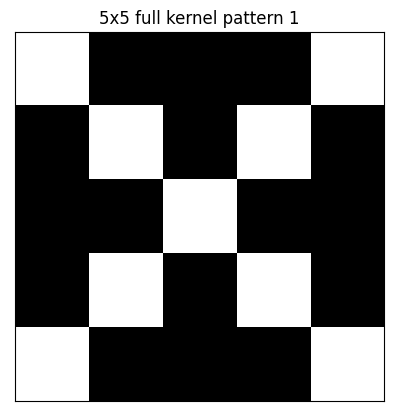
\includegraphics[width=0.33\textwidth]{../../code/serialization/kernels/5x5/full/5x5_kernel_full_1.png}
			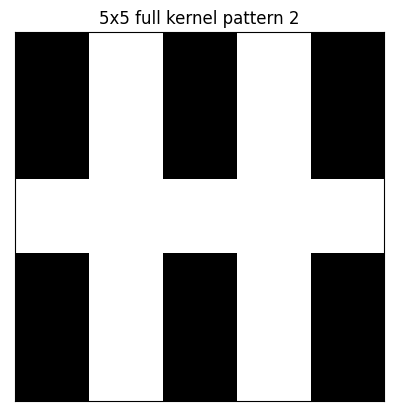
\includegraphics[width=0.33\textwidth]{../../code/serialization/kernels/5x5/full/5x5_kernel_full_2.png}
			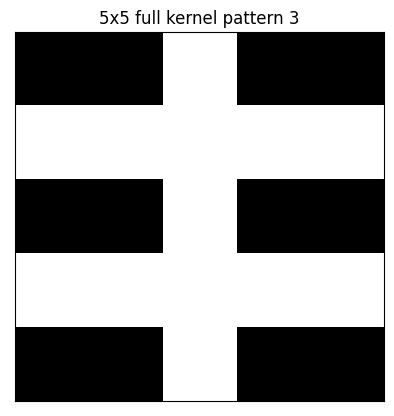
\includegraphics[width=0.33\textwidth]{../../code/serialization/kernels/5x5/full/5x5_kernel_full_3.png}
			\caption{Non-zero elements of $\ker{\Phi}$ for a $5 \times 5$ grid}
		\end{figure}
	
		We can partition the squares of the $5 \times 5$ grid to one of four regions based on which quiet patterns they are a part of.
		
		\begin{figure}[H]
			\centering
			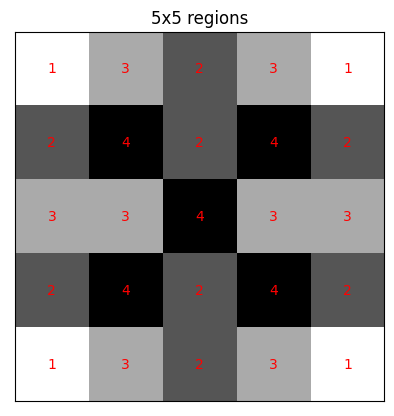
\includegraphics[width=0.49\textwidth]{../../code/serialization/regions/5x5_regions.png}
			\caption{The four regions of a $5 \times 5$ grid}
		\end{figure}
	
		Region 1 is the intersection of covers 2 and 3; region 2 is the intersection of  covers 1 and 2; region 3 is the intersection of covers 1 and 3;
		region 4 is the intersection of the complements.
		
		Let $Y$ be an initial configuration that requires the maximum number of clicks to solve.
		Let $X$ be a solution to $Y$ that uses the fewest clicks.
		Let $A$ be the number of vertices in $X$ in region 1, $B$ in region 2, $C$ in region 3, and $D$ in region 4.
		Then the solution uses $\abs{X} = A + B + C + D$ moves.
		
		If we apply quiet pattern 1, we obtain another solution that uses $A + (8 - B) + (8 - C) + D$ moves.
		Since we assumed $X$ was a minimal solution,
		\begin{equation*}
			A + B + C + D \leq A + (8 - B) + (8 - C) + D.
		\end{equation*}
		Rearranging,
		\begin{equation}\label{5x5_constr1}
			B + C \leq 8.
		\end{equation}
	
		If we apply quiet pattern 2, we obtain another solution that uses $(4 - A) + (8 - B) + C + D$ moves.
		Since we assumed $X$ was a minimal solution,
		\begin{equation*}
			A + B + C + D \leq (4 - A) + (8 - B) + C + D.
		\end{equation*}
		Rearranging,
		\begin{equation}\label{5x5_constr2}
			A + B \leq 6.
		\end{equation}
	
		If we apply quiet pattern 3, we obtain another solution that uses $(4 - A) + B + (8 - C) + D$ moves.
		Since we assumed $X$ was already a minimal solution,
		\begin{equation*}
			A + B + C + D \leq (4 - A) + B + (8 - C) + D.
		\end{equation*}
		Rearranging,
		\begin{equation}\label{5x5_constr3}
			A + C \leq 6.
		\end{equation}
	
		None of \eqref{5x5_constr1}, \eqref{5x5_constr2}, or \eqref{5x5_constr3} affect $D$.
		Thus, $D$ is not constrained beyond the fact that region 4 contains five vertices.
		Since we assumed the solution to $Y$ required as many clicks as possible, $D = 5$.
	
		Putting \eqref{5x5_constr1}, \eqref{5x5_constr2}, and \eqref{5x5_constr3} in matrix form,
		\begin{equation}\label{5x5_ilp}
			\begin{bmatrix}
				0 & 1 & 1 \\
				1 & 1 & 0 \\
				1 & 0 & 1
			\end{bmatrix}
			\begin{bmatrix}
				A \\
				B \\
				C
			\end{bmatrix}
			\leq
			\begin{bmatrix}
				8 \\
				6 \\
				6
			\end{bmatrix}.
		\end{equation}
		Thus, we need to solve this integer linear program (ILP), maximizing the $L^1$-norm $A + B + C$.
		
		Since all entries in the constraint matrix of \eqref{5x5_ilp} are non-negative, finding an integer solution where the constraints are tight (i.e. replace the $\leq$ in \eqref{5x5_ilp} with $=$) would be the solution to the ILP.
		
		Assuming the constraints are tight, we find that
		\begin{equation*}
			\begin{bmatrix}
				A \\
				B \\
				C
			\end{bmatrix}
			=
			\begin{bmatrix}
				2 \\
				4 \\
				4
			\end{bmatrix}
		\end{equation*}
		is the solution to the ILP.
		So, the solution to the Min Moves Problem for a $5 \times 5$ grid is $\abs{X} = A + B + C + D = 2 + 4 + 4 + 5 = 15$.
	\end{proof}

	\section{Inequality for Larger Grids}
	If we have an even parity cover for a smaller grid, we can construct an even parity cover for a larger grid.
	
	\begin{theorem}\label{tiling-quiet-patterns}
		Let $d(n) = \dim{\ker{\Phi}}$ for an $n \times n$ grid.
		Then for all $n,k \in \N$,
		\begin{equation*}
			d(nk - 1) \geq d(n-1).
		\end{equation*}
	\end{theorem}
	\begin{proof}
		Let $n,k \in \N$.
		Since $nk - 1 = k(n-1) + (k-1)$, an $(nk-1) \times (nk-1)$ grid consists of a $k \times k$ grid of $(n-1) \times (n-1)$ grids, each separated by a horizontal or vertical strip of height or width 1.
	
		Let $Q$ be an even parity cover for an $(n-1) \times (n-1)$ grid.
		Let $R$ be $Q$ tiled $k$ times horizontally and vertically onto an $(nk-1) \times (nk-1)$ grid, where each tile is a horizontal/vertical reflection of its horizontal/vertical neighboring tiles, as shown below.
		
		\begin{figure}[H]
			\centering
% Code the generate figure w/o Q's
%			\begin{tikzpicture}[scale=0.33]
%				\edef\M{3} % Width of each tile
%				\edef\K{5} % Number of tiles in each direction
%				\pgfmathparse{(\M+1)*\K - 1} % Size of large grid
%				\edef\N{\pgfmathresult}
%				
%				\draw[black,thin] (0,0) grid (\N,\N);
%				
%				\foreach \i in {1,2,...,\K}{
%					\foreach \j in {1,2,...,\K}{
%						\pgfmathparse{(\i - 1) * (\M + 1)}
%						\edef\X{\pgfmathresult}
%						\pgfmathparse{(\j - 1) * (\M + 1)}
%						\edef\Y{\pgfmathresult}
%						
%						\draw[fill,gray,opacity=0.707] (\X, \Y) rectangle (\X + \M, \Y + \M);
%						%\node at (\X + \M/2, \Y + \M/2) {$Q$};
%					}
%				}
%			\end{tikzpicture}
			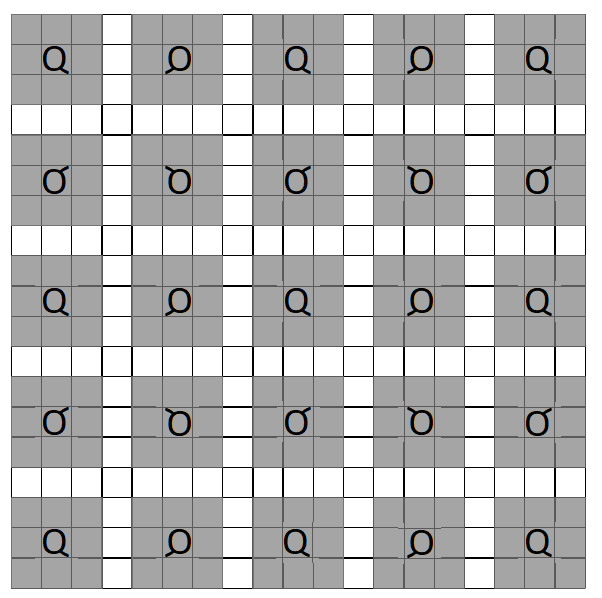
\includegraphics[width=0.5\textwidth]{tiling_q.png}
			\caption{Pattern $Q$ tiled 5 times.}	
		\end{figure}
	
		We will show that $R$ is an even parity cover of an $(nk - 1) \times (nk - 1)$ grid.
		Consider any vertex $v$ in the $(nk-1) \times (nk-1)$ grid.
		If $v$ is one of the areas containing a reflection of $Q$, then $N(v) \cap R$ is even because $Q$ is an even parity cover.
		If $v$ not one of these areas containing a reflection of $Q$, then $v \not\in Q$, and $N(v)$ contains either zero or two vertices that are in a reflection of $Q$.
		If $N(v)$ contains zero such vertices, then $\abs{N(v) \cap R} = 0$, which is even.
		If $N(v)$ contains two such vertices, then these vertices are either both in $R$ or neither are in $R$.
		Thus, $\abs{N(v) \cap R}$ is even.
		So, $R$ is an even parity cover.
		
		So, each even parity cover of an $(n-1) \times (n-1)$ grid allows us to generate a unique even parity cover for an $(nk-1) \times (nk-1)$ grid.
		Thus,
		\begin{equation*}
			d(nk-1) \geq d(n-1),
		\end{equation*}
		as desired.
	\end{proof}

	\section{Establishing an Upper Bound}
	Applying theorem \ref{tiling-quiet-patterns} for $n=6$, we get that for all $k \in \N$,
	\begin{equation*}
		d(6k - 1) \geq d(5) = 2.
	\end{equation*}
	For $(6k-1) \times (6k-1)$ grids, we know that we're tiling the $5 \times5 $ even parity covers.
	For example, notice how the $17 \times 17$ even parity covers are simply the $5 \times 5$ even parity covers tiled $k=3$ times.
	
	\begin{figure}[H]
		\centering
		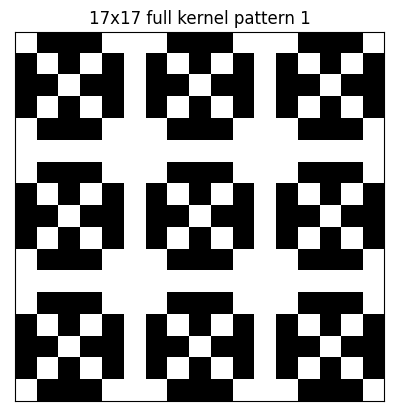
\includegraphics[width=0.33\textwidth]{../../code/serialization/kernels/17x17/full/17x17_kernel_full_1.png}
		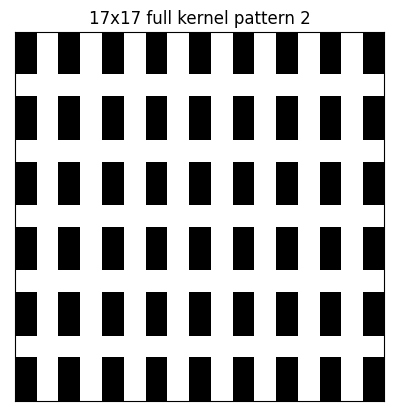
\includegraphics[width=0.33\textwidth]{../../code/serialization/kernels/17x17/full/17x17_kernel_full_2.png}
		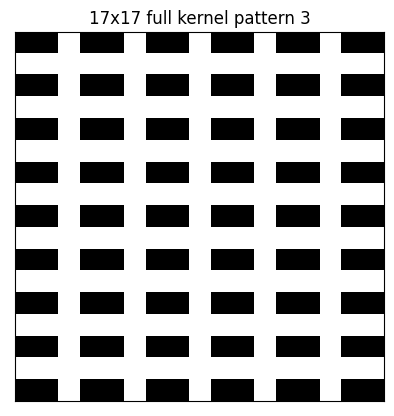
\includegraphics[width=0.33\textwidth]{../../code/serialization/kernels/17x17/full/17x17_kernel_full_3.png}
		\caption{Non-zero elements of $\ker{\Phi}$ for a $17 \times 17$ grid}
	\end{figure}
	
	Thus, we can apply the same proof technique as in theorem \ref{min-moves-problem-5x5} to find an upper bound for the Min Moves Problem for such grid sizes.
	We'll also know that if $d(6k - 1) = 2$, then this upper bound is exact, and we have solved the Min Moves Problem.
	
	\begin{theorem}\label{min-moves-problem-6k-1x6k-1}
		Let $k \in \N$.
		Then the solution to the MMP for a $(6k - 1) \times (6k - 1)$ grid is at most $26k^2 - 12k + 1$.
		This bound is exactly the solution to the MMP when $d(6k-1)=2$.
	\end{theorem}
	\begin{proof}
		Let $k \in \N$.
		Applying theorem \ref{tiling-quiet-patterns} with $n=6$, the even parity covers of the $5 \times 5$ grid will tile a $(6k - 1) \times (6k - 1)$ grid.
		We can partition the vertices of the grid into four regions based on which even parity covers they are a part of.
		Using the same numbering for even parity covers as in theorem \ref{min-moves-problem-5x5}, region 1 is the intersection of even parity covers 2 and 3; region 2 is the intersection of even parity covers 1 and 2; region 3 is the intersection of even parity covers 1 and 3; region 4 is the intersection of the complements.
		Region 1 contains $4k^2$ vertices, regions 2 and 3 contain $8k^2$ vertices, and region 4 contains the remaining $16k^2 - 12k + 1$ vertices.
		
		Let $Y$ be an initial configuration that requires the maximum number of clicks to solve.
		Let $X$ be a solution to $Y$ that uses the fewest clicks.
		Let $A$ be the number of moves in $X$ in region 1, $B$ in region 2, $C$ in region 3, and $D$ in region 4.
		Then the solution uses $\abs{X} = A + B + C + D$ moves.
		
		Applying the three even parity covers and deriving the constraints, we find that $D$ is unconstrained and can thus be set to $16k^2 - 12k + 1$, while $A$, $B$, and $C$ are constrained by the following ILP:
		\begin{equation}
			\begin{bmatrix}
				0 & 1 & 1 \\
				1 & 1 & 0 \\
				1 & 0 & 1 
			\end{bmatrix}
			\begin{bmatrix}
				A \\
				B \\
				C
			\end{bmatrix}
			\leq
			\begin{bmatrix}
				8 \\
				6 \\
				6
			\end{bmatrix}k^2.
		\end{equation}
		This is the exact same set of constraints as in theorem \ref{min-moves-problem-5x5}, just with a factor of $k^2$.
		Thus,
		\begin{equation*}
			\begin{bmatrix}
				A \\
				B \\
				C
			\end{bmatrix}
			=
			\begin{bmatrix}
				2 \\
				4 \\
				4
			\end{bmatrix}k^2.
		\end{equation*}
		is the solution to the ILP.
		Thus, $\abs{X} = A + B + C + D = 2k^2 + 4k^2 +  4k^2 + 16k^2 - 12k + 1 = 26k^2 - 12k + 1$.
		
		If $\dim{\ker{\Phi}} = 2$, we have considered all even parity covers and have solved the MMP.
		However, if $\dim{\ker{\Phi}} > 2$ there will be more even parity covers that give rise to more and more restrictive constraints, meaning we have an upper bound.
	\end{proof}

	The $5 \times 5$, $17 \times 17$, $41 \times 41$, $53 \times 53$, $77 \times 77$, $113 \times 113$, $\dots$ grids are those of size $(6k-1) \times (6k-1)$ with nullity 2.
	Thus, we find that the solutions to the MMP for these grids are 15, 199, 1191, 1999, 4239, 9159, $\dots$ respectively.
	
	\section{Conjectures}
	\begin{conjecture}\label{all-nullity2-conj}
		If an $n \times n$ grid has nullity 2, then $n \equiv -1 \mod 6$.
	\end{conjecture}
	That is, the quiet patterns of all nullity 2 grids are tilings of the $5 \times 5$ quiet patterns.
	If true, this would mean that we have solved the MMP for all nullity 2 grids.

	\begin{conjecture}\label{ilp-conj}
		The proof technique of assuming our integer program can be solved with all constraints tight will only work for grids with nullity 2, none higher.
	\end{conjecture}
	That is, solving the ILP by assuming all constraints can be tightly satisfied does not work for grids with nullity greater than 2.
	
	\section{Future Work}
	We'd like future work to focus on resolving conjecture \ref{all-nullity2-conj} and solving the MMP on grids with nullities greater than 2.
	For any sized grid (in fact, any graph), we can apply the same technique as in theorems \ref{min-moves-problem-5x5} and \ref{min-moves-problem-6k-1x6k-1} of finding the solution to the Min Moves Problem as the solution to an ILP.
	However, as we state in conjecture \ref{ilp-conj}, it seems the ILP for larger nullities cannot be solved with all constraints tight.
	The $4 \times 4$ grid with nullity 4 (nullities are always even) is the smallest with nullity greater than 2.
	We know via brute force that the answer to the Min Moves Problem in this case is 7.
	Perhaps if we better understood how to solve the ILP for the $4 \times 4$ grid, we could generalize to larger grids.
	
	We'd also like future work to focus more on understanding the relationships between the nullities of different sized grids.
	The inequality derived in theorem \ref{tiling-quiet-patterns} is a good start to this, but there seem to be many other patterns to discover.
	For example, Sutner conjectures in \cite{Sutner1989} that $d(2n+1) = 2d(n) + \delta_n$, where $\delta_n \in \{0,2\}$, and $\delta_{2n+1} = \delta_n$.

	\newpage
	\bibliography{refs.bib}
	\bibliographystyle{amsplain}
\end{document}